\documentclass[a4paper]{article}

%% Language and font encodings
\usepackage[english]{babel}
\usepackage[utf8x]{inputenc}
\usepackage[T1]{fontenc}

%% Sets page size and margins
\usepackage[a4paper,top=3cm,bottom=2cm,left=3cm,right=3cm,marginparwidth=1.75cm]{geometry}

%% Useful packages
\usepackage{amsmath}
\usepackage{graphicx}
\usepackage[colorinlistoftodos]{todonotes}
\usepackage[colorlinks=true, allcolors=blue]{hyperref}
\usepackage[ampersand]{easylist}
\ListProperties(Hide=100, Hang=true, Progressive=3ex, Style*=$\bullet$ ,
Style2*=-- ,Style3*=$\circ$ ,Style4*=\tiny$\blacksquare$ )

\title{FCC Documentation}
\author{Daniel Deutsch}

\begin{document}
\maketitle

\begin{abstract}
My documentation and proposals for the FCC Meetup Vienna. Written in LaTex!
\end{abstract}

\section{Objectives and Values of the FCC Meetup}
Connecting people with similar ambitions in real life and provide a platform for exchange and improvement


\section{Subject}
FCC - Programming, web development enthusiasts from beginner to expert.

\section{Team}
\begin{itemize}
\item Robert as founder and host
\item Daniel and Lukas as co-host
\end{itemize}

\section{Basics}
\begin{itemize}
\item Location: Coworking spaces, that provide space for free. (eg Sector5)
\item Timescheduling: Reconciliation between the hosts and scheduled between other development events. Also dependent on availability of the provided space.
\end{itemize}

\section{Online Communication}
\begin{itemize}
\item meetup.com - for setting framework and information
\item facebook - for nourishing community and provide information
\item twitter - recent updates in the community
\end{itemize}

\section{Promoting Events}
\begin{itemize}
\item Mail on meetup.com?
\item Posts in Social Media
\end{itemize}

\section{Program}
\begin{easylist}
& Showcase
  && A person guiding the audience through a codebase they are currently working on.
& Discussion Circle
  && Setting different topics and letting the audience discuss.
& Presentations
  && Different topics with following QA
& Coding Sessions
  && Mob Sessions
  && FCC Codes
  && Other small Algorithms
\end{easylist}

\section{Sponsors}
Always open and on the search for sponsors. Easier when we have a community established.

\section{Checklist at the Event}
\begin{easylist}
& Before the Meetup
&& Come 30–45 min early and introduce yourself to the location host
&& Make sure it’s obvious to find the location or put up navigational signs
&& If you have a co-organiser, one of you should be welcoming attendees
&& Setup the location (stage, chairs)
&& Test the projector
&& sync with speakers who wants to go first
&& prepare a short slide deck with the schedule and the logos of the sponsors
&& let the sponsors speak for 2–3 minutes

& During the Meetup
&& in a smaller group let everyone introduce themselves to connect (start with yourself to lead by example)
&& make sure one of your co-organisers or you moderate the event
&& have fun and enjoy

& After the Meetup
&& after the last talk thank everybody for coming and how long they can stay
&& clean up the location
&& personally thank the location host
\end{easylist}

\begin{figure}
\centering
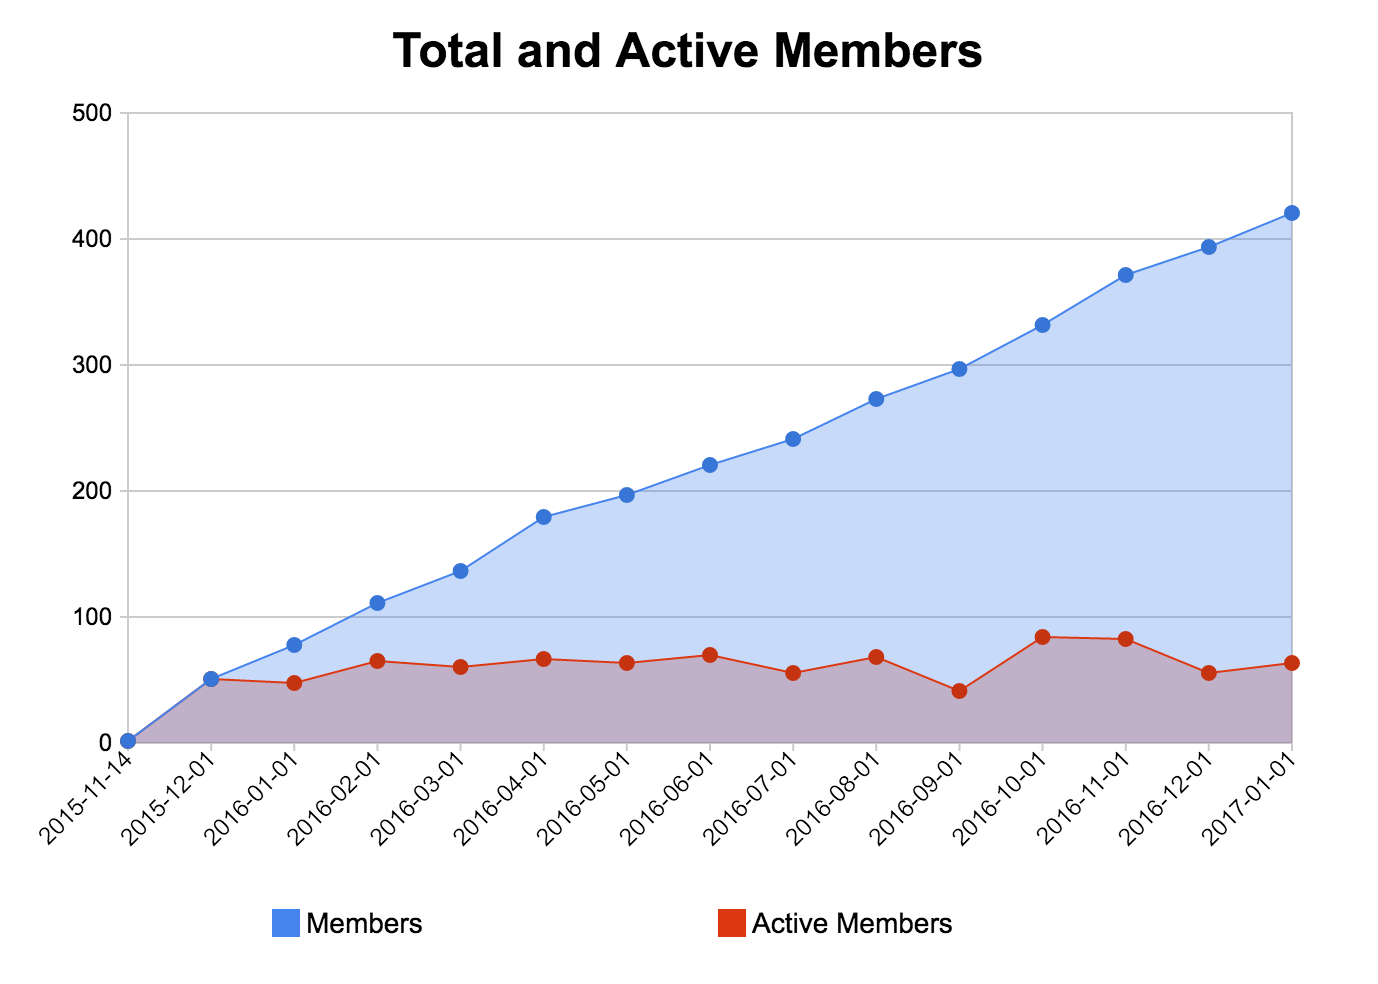
\includegraphics[width=0.3\textwidth]{graph_fcc.jpeg}
\caption{\label{fig:graph_fcc}Current Statistic of Memebers}
\end{figure}

\section{ToDo}
\begin{enumerate}
\item Set scope of duties for each co hosts.
\item Whats our current booking status?
\item Provide draft for monthly meetup.
\item Create a special FCC Vienna Image used for logos etc. (Maybe find designer if necessary - simple banner and logo)
\item Establish a quarterly meeting between hosts to analyze past meetings and set new standards for future meetups.
\item Refactor Github Repo ( Manage Team abilities, provide documents of meetups)
\item Revaluate Meetup.com settings
\item Maybe develop a facebook/twitter strategy?
\item Establish Feedback loop from visitors!!!!!!!!
\end{enumerate}



\section{Ideas for the Meetup in February}
\begin{easylist}
& Introduction
& Talk about FCC - Maybe Presentation and Overview over FCC
& Discussion Circle/Programming
& Feedback
& Additional: Moderating the Event!
\end{easylist}

\end{document}
% * <ddeutsch1@gmx.at> 2017-01-22T16:35:13.731Z:
%
% ^.
% * <ddeutsch1@gmx.at> 2017-01-22T16:35:12.957Z:
%
% ^.
% * <ddeutsch1@gmx.at> 2017-01-22T16:35:10.725Z:
%
% ^.
